\documentclass{beamer}

\usetheme{zg}
\usepackage{ulem}

\title{Spring}
\date{\today}
\author{Fernando Camargo}
\institute{ZG Soluções}


\begin{document}
\maketitle

\section{O que é Spring?}

\begin{frame}{O que é Spring?}
 \begin{outline}
  \1<1-> Mais popular framework para desenvolvimento \only<1>{Java}\only<2->{\sout{Java} na JVM}
  \1<3-> Objetivos
    \2<3-> Simplificar o desenvolvimento em JEE
    \2<4-> Facilitar as tarefas comuns (inúmeros módulos disponíveis)
    \2<5-> Promover boas práticas de desenvolvimento
    \2<6-> Código fácil de testar e de manter
  \1<7-> Spring Boot para começar rápido um projeto
 \end{outline}
\end{frame}

\begin{frame}{Estratégias chaves}
 \begin{outline}
  \1<1-> Uso de POJOs
    \2 Leve
    \2 Minimamente invasivo
  \1<2-> Baixo acoplamento
    \2 Injeção de dependências
    \2 Interfaces
  \1<3-> Programação declarativa
    \2 Aspectos
    \2 Convenções comuns
  \1<4-> Eliminação de código "chiclê"
    \2 Aspectos
    \2 Templates
 \end{outline}
\end{frame}

\section{Arquitetura}

\begin{frame}{Arquitetura}
  \begin{center}
    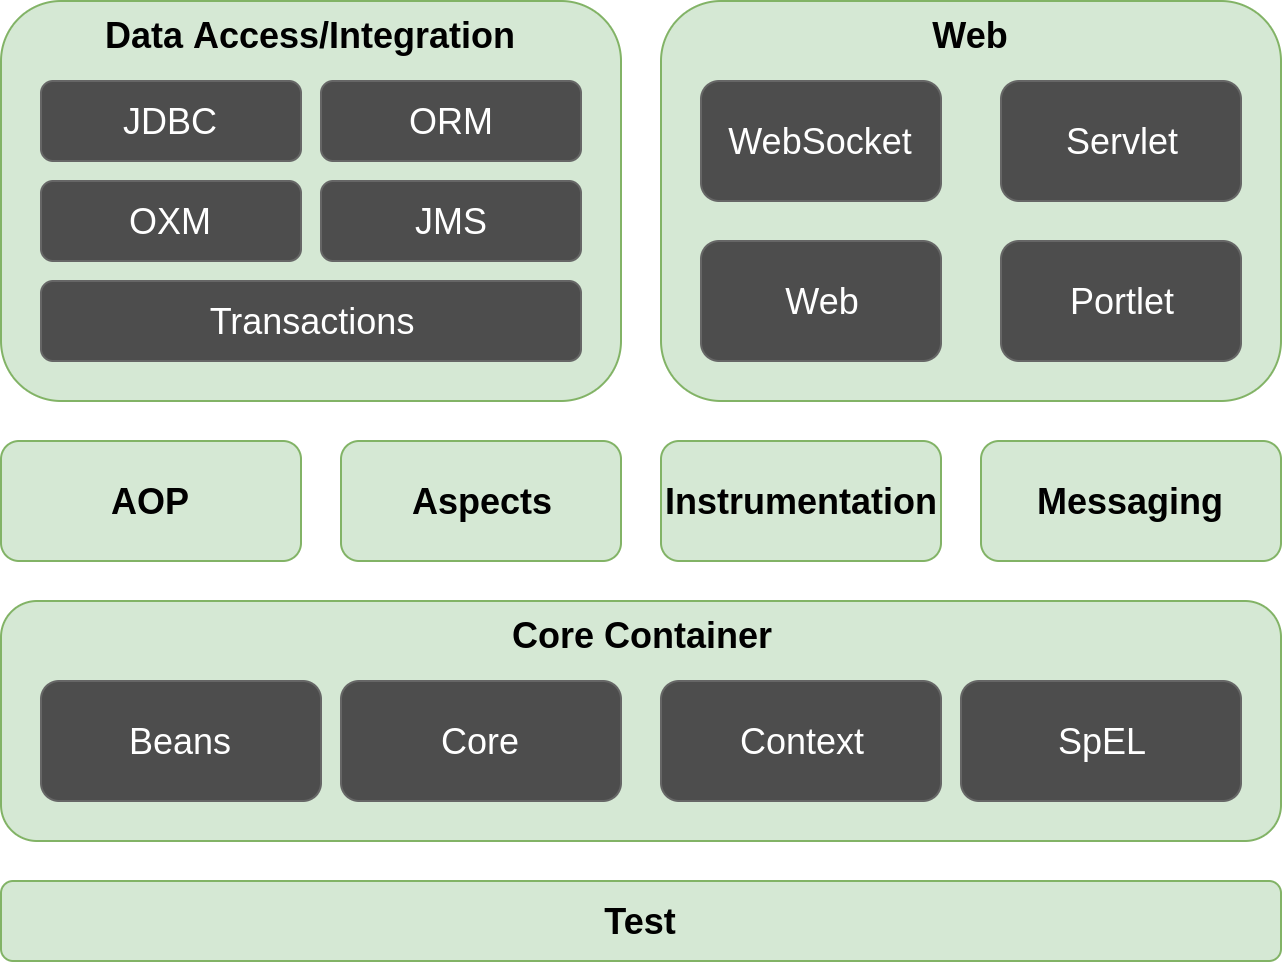
\includegraphics[width=\textwidth]{arquitetura-spring}
  \end{center}
\end{frame}

\begin{frame}{Core Container}
 \begin{outline}
  \1<1-> \textbf{Core} (spring-core) e \textbf{Bean} (spring-beans)
    \2 Parte fundamental do framework
    \2 Inversão de Controle (IoC) e Injeção de Dependências (DI)
  \1<2-> \textbf{Context} (spring-context) $\rightarrow$ acesso a objetos definidos e configurados
  \1<3-> \textbf{SpEL} (spring-expression)
    \2 Linguagem de Expressão (EL)
    \2 Busca e manipulação de um objeto
 \end{outline}
\end{frame}

\begin{frame}{Data Access/Integration}
 \begin{outline}
  \1<1-> \textbf{JDBC} (spring-jdbc) $\rightarrow$ camada de abstração sob JDBC
  \1<2-> \textbf{Transaction} (spring-tx) $\rightarrow$ gerenciamento de transações
    \2 Programática
    \2 Declarativa
  \1<3-> \textbf{ORM} (spring-orm)
    \2 Camada de abstração para populares ORMs (JPA, Hibernate, etc.)
    \2 Permite integrar com outras funcionalidades do Spring, como \textbf{Transaction}
  \1<4-> \textbf{OXM} (spring-oxm)
    \2 Camada de abstração para Mapeamento Objeto/XML
    \2 Suporta implementações como JAXB, Castor, XMLBeans, etc.
  \1<4-> \textbf{JMS} (spring-jms) $\rightarrow$ serviço de mensagens
 \end{outline}
\end{frame}

\begin{frame}{Web}
 \begin{outline}
  \1<1-> \textbf{Web} (spring-web)
    \2 Inicialização do IoC para Web
    \2 Utilitários Web
  \1<2-> \textbf{Servlet} (spring-webmvc)
    \2 Spring MVC $\rightarrow$ framework web
    \2 REST Web Services
  \1<3-> \textbf{Portlet} (spring-webmvc-portlet) $\rightarrow$ Spring MVC para Portlets
  \1<2-> \textbf{WebSocket} (spring-websocket) $\rightarrow$ suporte a WebSocket
 \end{outline}
\end{frame}

\begin{frame}{Diversos}
 \begin{outline}
  \1<1-> \textbf{AOP} (spring-aop) $\rightarrow$ implementação de Programação Orientada a Aspectos
  \1<2-> \textbf{Aspects} (spring-aspects) $\rightarrow$ integração com AspectJ
  \1<3-> \textbf{Instrumentation} (spring-instrument)
    \2 Suporte a instrumentação de classes
    \2 Implementação de Class Loaders para certo servidores
  \1<4-> \textbf{Test} (spring-test) $\rightarrow$ suporte a testes com JUnit e TestNG para aplicações Spring
 \end{outline}
\end{frame}

\section{Conceitos de base}

\begin{frame}{Injeção de Dependências (DI)}
 \begin{outline}
  \1<1-> Separa a criação de dependências de uma classe de seu comportamento
  \1<2-> Reduz o acoplamento e aumenta coesão
 \end{outline}
 \begin{center}
  \visible<3->{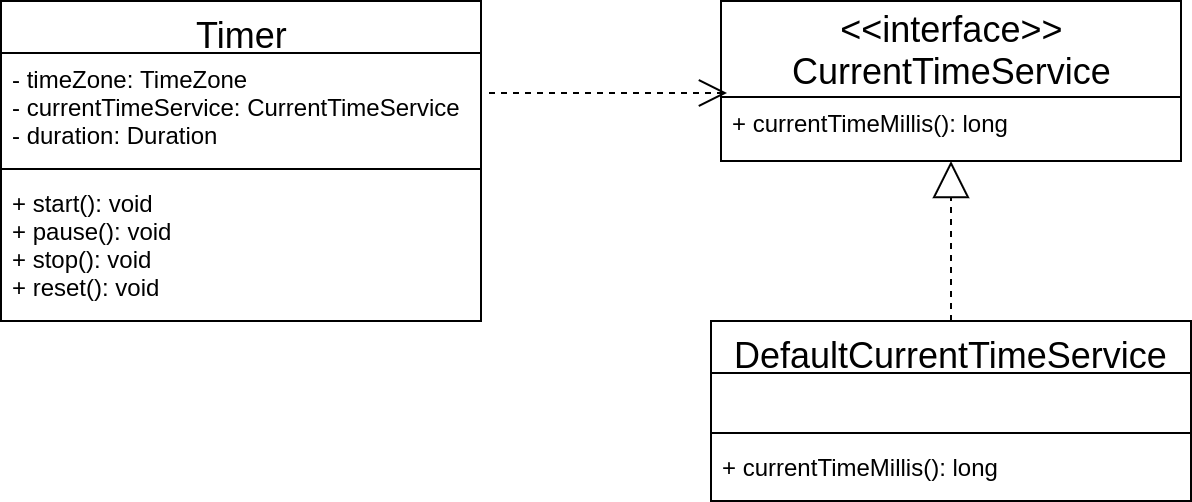
\includegraphics[width=\textwidth]{diagrama-injecao-dependencias}}
 \end{center}
\end{frame}

\begin{frame}[fragile]{Exemplo sem injeção de dependências}
 \begin{minted}[fontsize=\tiny]{java}
public class Timer {

  private CurrentTimeService currentTimeService;
  private TimeZone timeZone;

  public Timer(){
    currentTimeService = new DefaultCurrentTimeService();
    timeZone = TimeZone.getDefault();
  }

  public void start(){
    // Faz uso de CurrentTimeService e TimeZone
  }
  
  // ...

}

// Uso do Timer
Timer timer = new Timer();
timer.start();
  \end{minted}
\end{frame}

\begin{frame}[fragile]{Exemplo com injeção de dependências}
 \begin{minted}[fontsize=\tiny]{java}
public class Timer {

  private CurrentTimeService currentTimeService;
  private TimeZone timeZone;

  public Timer(CurrentTimeService currentTimeService, TimeZone timeZone){
    currentTimeService = currentTimeService;
    timeZone = timeZone;
  }

  public void start(){
    // Faz uso de CurrentTimeService e TimeZone
  }
  
  // ...

}

// Uso do Timer
CurrentTimeService currentTimeService = new DefaultCurrentTimeService();
TimeZone timeZone = TimeZone.getDefault();

Timer timer = new Timer(currentTimeService, timeZone);
timer.start();
  \end{minted}
\end{frame}

\begin{frame}[fragile]{Exemplo de teste com injeção de dependências}
 \begin{minted}[fontsize=\tiny]{java}
public class Timer {

  private CurrentTimeService currentTimeService;
  private TimeZone timeZone;

  public Timer(CurrentTimeService currentTimeService, TimeZone timeZone){
    currentTimeService = currentTimeService;
    timeZone = timeZone;
  }

  public void start(){
    // Faz uso de CurrentTimeService e TimeZone
  }
  
  // ...

}

// Teste do Timer
StubCurrentTimeService currentTimeService = new StubCurrentTimeService();
TimeZone timeZone = TimeZone.getTimeZone("America/Sao_Paulo");

Timer timer = new Timer(currentTimeService, timeZone);
timer.start();

// Ajuste de tempo simulado
currentTimeService.tick(5, TimeUnit.SECONDS);
  \end{minted}
\end{frame}

\begin{frame}{Injeção de Dependências (DI)}
 \begin{outline}
  \1<1-> Mesmo a injeção de dependências mais básica (sem frameworks) já apresenta benefícios
    \1<2-> Quem vai criar toda estrutura de objetos?
  \1<3-> Existem muitos frameworks de injeção de dependência
    \2 Spring
    \2 CDI/EJB
    \2 Guice
    \2 Dagger
    \2 etc.
  \1<4-> Um container é responsável pela construção dos objetos (e suas dependências)
    \2 Main: "Me dê um Timer"
    \2 Container: "Só um momento, o Timer tem duas dependências, vou criá-las como configurado e te retornar um Timer totalmente funcional."
 \end{outline}
\end{frame}

\begin{frame}{Inversão de Controle (IoC)}
 \begin{outline}
  \1<1-> Princípio de Hollywood: "Não nos chame, nós o chamaremos"
  \1<2-> Tradicional: código criado possui todas responsabilidades
    \2<3-> Constrói suas dependências
    \2<4-> Gerencia seu próprio ciclo de vida
    \2<5-> Executa lógica de negócios
  \1<6-> IoC: separação de responsabilidades
    \2 Container gerencia ciclo de vida, além de contruir e injetar dependências
    \2 Código criado executa lógica de negócios
 \end{outline}
\end{frame}

\begin{frame}{Bean}
 Todo objeto da aplicação, gerenciado pelo Container do Spring, é chamado \alert{bean}.
 \begin{center}
   \only<1>{
\includegraphics[width=0.6\textwidth]{mr-bean}}
   \only<2>{
\includegraphics[width=0.6\textwidth]{beans}}
 \end{center}
\end{frame}

\section{Spring IoC}

\begin{frame}{Spring IoC}
  \begin{center}
    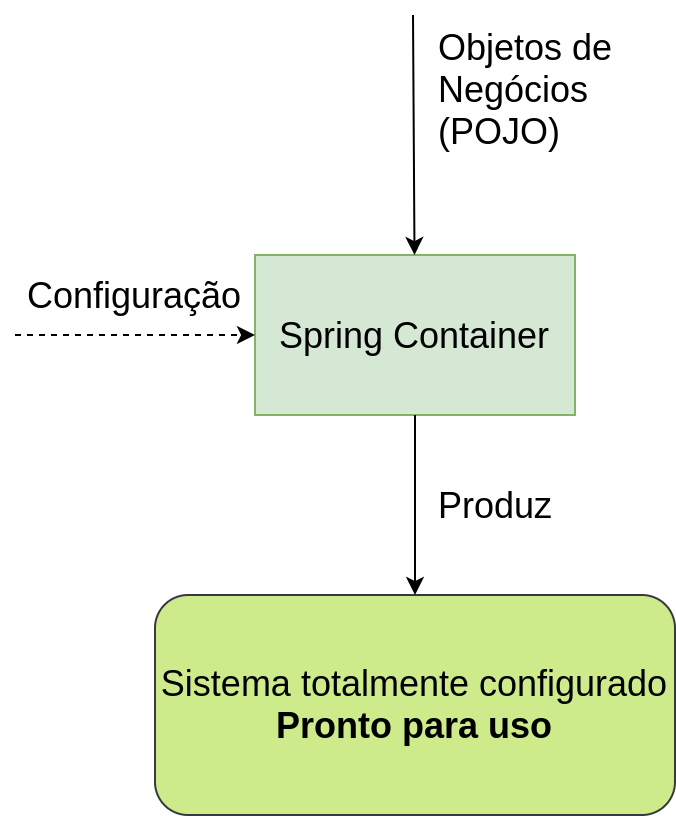
\includegraphics[width=0.6\textwidth]{spring-container}
  \end{center}
\end{frame}

\begin{frame}{Componentes do Spring IoC}
 \begin{outline}
  \1<1-> \textbf{BeanFactory}
    \2<1-> Avançado mecanismo de configuração capaz de gerenciar qualquer tipo de objeto
    \2<2-> Responsável pela criação e injeção de beans
  \1<3-> \textbf{ApplicationContext}
    \2<3-> Sub-interface de \textbf{BeanFactory}, adicionando:
      \3<3-> Integração mais fácil com funcionalidades do Spring AOP
      \3<4-> Internacionalização de mensagens
      \3<5-> Publicação de eventos
      \3<6-> Contextos específicos para a camada de aplicação (\textbf{WebApplicationContext} para Web, por exemplo)
    \2<7-> Representa o Container
    \2<8-> Obtém configurações via metadados: XML, Annotations ou Código de configuração
 \end{outline}
\end{frame}

\begin{frame}{Implementações do ApplicationContext}
 \begin{outline}
  \1 ClassPathXmlApplicationContext
  \1 FileSystemXmlApplicationContext
  \1 XmlWebApplicationContext
  \1 AnnotationConfigApplicationContext
  \1 AnnotationConfigWebApplicationContext
 \end{outline}
\end{frame}

\begin{frame}{Opções de Configuração}
 \begin{outline}
  \1<1-> Configuração explícita via XML
  \1<2-> Configuração explícita via Java
  \1<3-> Configuração implícita via descoberta e conexão automática de beans
 \end{outline}
\end{frame}

\subsection{Descoberta automática de beans}

\begin{frame}{Descoberta automática de beans}
 \begin{outline}
  \1<1-> \textbf{Component scanning}: automaticamente descobre beans a serem criados no ApplicationContext
  \1<2-> \textbf{Autowiring}: automaticamente satisfaz dependências dos beans
 \end{outline}
\end{frame}

\begin{frame}[fragile]{Exemplo Bean auto descoberto e injetado}
 \begin{minted}[fontsize=\tiny]{java}
@Service
public class SimpleMovieLister {

  private MovieFinder movieFinder;

  @Autowired
  public SimpleMovieLister(MovieFinder movieFinder) {
    this.movieFinder = movieFinder;
  }
  
  // ...

}
  \end{minted}
\end{frame}

\begin{frame}[fragile]{Habilitando auto descoberta via Java}
 \begin{minted}[fontsize=\tiny]{java}
@Configuration
@ComponentScan("org.example")
public class AppConfig  {
    // ...
}
  \end{minted}
\end{frame}

\begin{frame}[fragile]{Habilitando auto descoberta via XML}
 \begin{minted}[fontsize=\tiny]{xml}
<?xml version="1.0" encoding="UTF-8"?>
<beans xmlns="http://www.springframework.org/schema/beans"
    xmlns:xsi="http://www.w3.org/2001/XMLSchema-instance"
    xmlns:context="http://www.springframework.org/schema/context"
    xsi:schemaLocation="http://www.springframework.org/schema/beans
        http://www.springframework.org/schema/beans/spring-beans.xsd
        http://www.springframework.org/schema/context
        http://www.springframework.org/schema/context/spring-context.xsd">

    <context:component-scan base-package="org.example"/>

</beans>
  \end{minted}
\end{frame}

\begin{frame}{Definindo Beans via Annotations}
 \begin{outline}
  \1<1-> \alert{@Component("beanName")}
    \2<2-> \alert{@Service("beanName")}
    \2<3-> \alert{@Repository("beanName")}
    \2<4-> \alert{@Controller("beanName")}
  \1<5-> \alert{@Named("beanName")} $\rightarrow$ anotação definida pelo CDI e suportada pelo Spring
  \1<5-> Bean dectectado possuirá um nome que o identifique
  \1<6-> Se nome não especificado, utiliza-se nome da classe (primeira letra minúscula)
 \end{outline}
\end{frame}

\subsection{Definição de dependências}

\begin{frame}{Definindo dependências via Annotations}
 \begin{outline}
  \1<1-> \alert{@Autowired}
    \2<2-> Injeção via Construtor: todos parâmetros são injetados
    \2<3-> Injeção via Setter: setters anotados usados na injeção \textbf{após contrução}
    \2<4-> Injeção via Propriedade: propriedades anotadas são injetadas \textbf{após contrução}
  \1<5-> \alert{@Inject}
    \2<5-> Anotação definida pelo CDI e suportada pelo Spring
    \2<6-> Mesmo funcionamento de \alert{@Autowired}, mas com limitações
  \1<7-> \alert{@Value("property.name")}
    \2<7-> Injeta valores carregador de arquivos .properties
    \2<8-> Mesmos métodos de injeção do \alert{@Autowired}
 \end{outline}
\end{frame}

\begin{frame}[fragile]{Injeção via Construtor}
 \begin{minted}[fontsize=\tiny]{java}
@Service
public class SimpleMovieLister {

  private MovieFinder movieFinder;

  @Autowired
  public SimpleMovieLister(MovieFinder movieFinder) {
    this.movieFinder = movieFinder;
  }

  // ...
  
}
  \end{minted}
\end{frame}

\begin{frame}[fragile]{Injeção via Setter}
 \begin{minted}[fontsize=\tiny]{java}
@Service
public class SimpleMovieLister {

  private MovieFinder movieFinder;
  
  @Autowired
  public void setMovieFinder(MovieFinder movieFinder) {
    this.movieFinder = movieFinder;
  }

  // ...
  
}
  \end{minted}
\end{frame}

\begin{frame}[fragile]{Injeção via Propriedade}
 \begin{minted}[fontsize=\tiny]{java}
@Service
public class SimpleMovieLister {

  @Autowired
  private MovieFinder movieFinder;

  // ...
  
}
  \end{minted}
\end{frame}

\subsubsection{Qualificadores}

\begin{frame}{Seleção de dependências}
 \begin{outline}
  \1<1-> @Autowired de uma interface/classe abstrata:
    \2 Se existir uma única implementação, ela é utilizada
    \2 Se existirem múltiplas implementações, é necessário uma especificação: \alert{@Qualifier}
 \end{outline}
\end{frame}

\begin{frame}[fragile]{@Qualifier com beanName}
 \begin{minted}[fontsize=\tiny]{java}
@Service
public class MainMovieCatalog implements MovieCatalog {
  // ...
}

@Service
public class MovieRecommender {

  @Autowired
  @Qualifier("mainMovieCatalog")
  private MovieCatalog movieCatalog;

  // ...

}
  \end{minted}
\end{frame}

\begin{frame}[fragile]{@Qualifier com característica}
 \begin{minted}[fontsize=\tiny]{java}
@Service
@Qualifier("main")
public class MainMovieCatalog implements MovieCatalog {
  // ...
}

@Service
public class MovieRecommender {

  @Autowired
  @Qualifier("main")
  private MovieCatalog movieCatalog;

  // ...

}
  \end{minted}
\end{frame}

\begin{frame}[fragile]{@Qualifier com Custom Annotation}
 \begin{minted}[fontsize=\tiny]{java}
@Target({ElementType.FIELD, ElementType.PARAMETER})
@Retention(RetentionPolicy.RUNTIME)
@Qualifier
public @interface Main {
    
}

@Service
@Main
public class MainMovieCatalog implements MovieCatalog {
  // ...
}

@Service
public class MovieRecommender {

  @Autowired
  @Main
  private MovieCatalog movieCatalog;

  // ...

}
  \end{minted}
\end{frame}

\begin{frame}[fragile]{@Qualifier com Custom Annotation e valor}
 \begin{minted}[fontsize=\tiny]{java}
@Target({ElementType.FIELD, ElementType.PARAMETER})
@Retention(RetentionPolicy.RUNTIME)
@Qualifier
public @interface Genre {
    String value();
}

@Service
@Genre("action")
public class ActionMovieCatalog implements MovieCatalog {
  // ...
}

@Service
public class MovieRecommender {

  @Autowired
  @Genre("action")
  private MovieCatalog movieCatalog;

  // ...
  
}
  \end{minted}
\end{frame}

\begin{frame}[fragile]{@Qualifier com Custom Annotation e valores}
 \begin{minted}[fontsize=\tiny]{java}
@Target({ElementType.FIELD, ElementType.PARAMETER})
@Retention(RetentionPolicy.RUNTIME)
@Qualifier
public @interface MovieQualifier {
    String genre();
    String format();
}

@Service
@MovieQualifier(genre="action", format="dvd")
public class ActionMovieCatalog implements MovieCatalog {
  // ...
}

@Service
public class MovieRecommender {

  @Autowired
  @MovieQualifier(genre="action", format="dvd")
  private MovieCatalog movieCatalog;

  // ...
  
}
  \end{minted}
\end{frame}

\subsection{Registrando Beans diretamente}

\begin{frame}{Registrando Beans diretamente}
 \begin{outline}
  \1<1-> Além de auto detectados, beans também podem ser declarados
    \2 Via XML
    \2 Via Java (@Bean)
  \1<2-> Essas declarações também incluem injeção de dependência, referenciando outros beans
 \end{outline}
\end{frame}

\begin{frame}[fragile]{Registrando Beans via XML}
 \begin{minted}[fontsize=\tiny]{xml}
<?xml version="1.0" encoding="UTF-8"?>
<beans xmlns="http://www.springframework.org/schema/beans"
    xmlns:xsi="http://www.w3.org/2001/XMLSchema-instance"
    xmlns:context="http://www.springframework.org/schema/context"
    xsi:schemaLocation="http://www.springframework.org/schema/beans
        http://www.springframework.org/schema/beans/spring-beans.xsd
        http://www.springframework.org/schema/context
        http://www.springframework.org/schema/context/spring-context.xsd">

  <bean id="accountRepository" class="com.acme.AccountRepositoryImpl" />
        
  <bean id="transferService" class="com.acme.TransferServiceImpl">
    <constructor-arg ref="accountRepository" />
  </bean>

</beans>
  \end{minted}
\end{frame}

\begin{frame}[fragile]{Registrando Beans via Java}
 \begin{minted}[fontsize=\tiny]{java}
@Configuration
public class AppConfig {

  @Bean
  public AccountRepository accountRepository() {
    new AccountRepositoryImpl();
  }

  @Bean
  public TransferService transferService(AccountRepository accountRepository) {
    return new TransferServiceImpl(accountRepository);
  }

}
  \end{minted}
\end{frame}

\subsection{Ciclo de Vida}

\begin{frame}{Ciclo de Vida}
 \begin{center}
    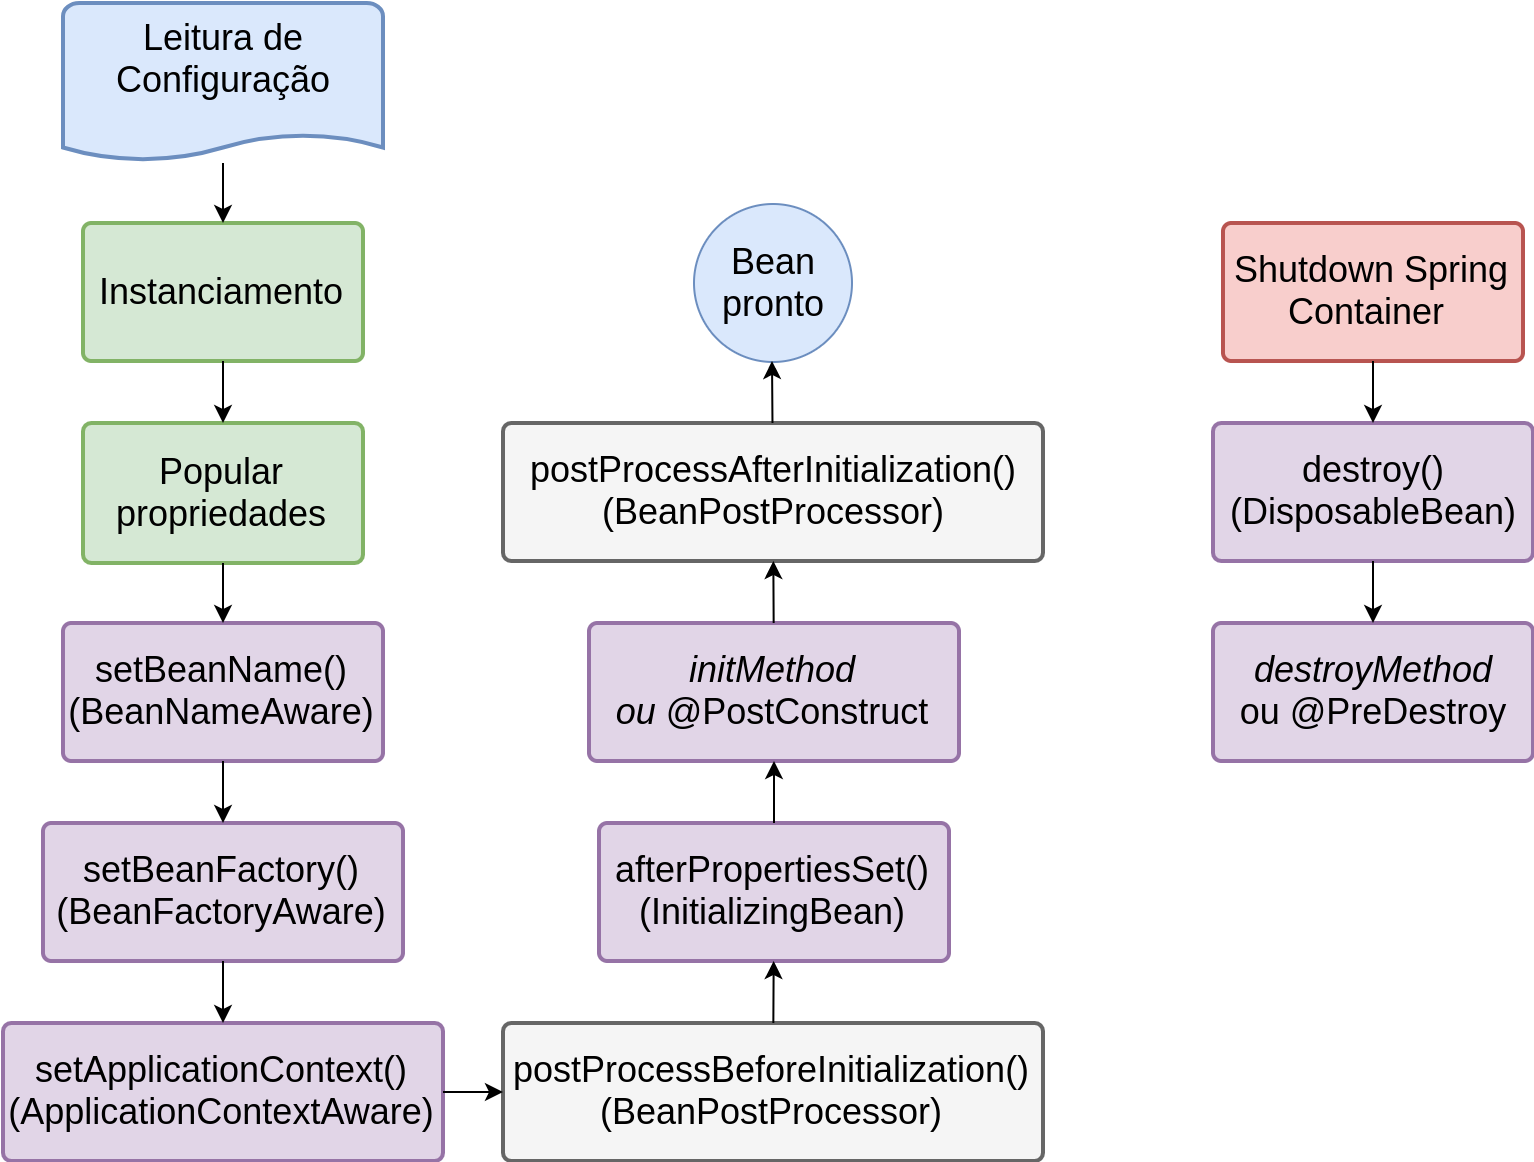
\includegraphics[width=0.9\textwidth]{ciclo-de-vida}
  \end{center}
\end{frame}

\subsection{Escopo de Vida}

\begin{frame}{Escopo de Vida}
 \begin{table}[]
  \begin{tabular}{@{}ll@{}}
    \toprule
    Escopo             & Descrição                                           \\ \midrule
    Singleton (Padrão) & Única instância criada e mantida pelo Container     \\
    Prototype          & Múltiplas instâncias criadas                        \\
    Request            & Única instância criada por requisição               \\
    Session            & Única instância criada por sessão                   \\ \bottomrule
  \end{tabular}
 \end{table}
\end{frame}

\begin{frame}[fragile]{@Scope}
 \begin{minted}[fontsize=\tiny]{java}
@Service
@Scope("prototype")
public class MovieRecommender {

  @Autowired
  private MovieCatalog movieCatalog;

  // ...
  
}
  \end{minted}
\end{frame}


\end{document}